% Template cho một chương

\chapter{Neural Structured Learning With Python/TensorFlow} % Tên của chương

\label{Chapter2} % Thay X bằng số chương tương ứng; để trích dẫn chương này ở chỗ nào đó trong bài, hãy sử dụng lệnh \ref{ChapterX} 

%----------------------------------------------------------------------------------------
%	MỤC 1
%----------------------------------------------------------------------------------------
\newcommand{\keyword}[1]{\textbf{#1}}
\newcommand{\tabhead}[1]{\textbf{#1}}
\newcommand{\code}[1]{\texttt{#1}}
\newcommand{\file}[1]{\texttt{\bfseries#1}}
\newcommand{\option}[1]{\texttt{\itshape#1}}


\section{Neural Structured Learning}
Neural Structured Learning (NSL) là một mô hình học tập mới để huấn luyện mạng thần kinh bằng cách tận dụng các tín hiệu có cấu trúc bên cạnh các đầu vào tính 
năng. Cấu trúc có thể rõ ràng như được biểu thị bằng biểu đồ hoặc ẩn khi gây ra "nhiễu loạn đối nghich.

Các tín hiệu có cấu trúc thường được sử dụng để biểu thị các mối quan hệ hoặc sự giống nhau giữa các mẫu có thể được gắn nhãn hoặc không gắn nhãn. Do đó, việc 
tận dụng các tín hiệu này trong quá trình huấn luyện mạng thần kinh sẽ khai thác cả dữ liệu được gắn nhãn và không được gắn nhãn, điều này có thể cải thiện độ 
chính xác của mô hình, đặc biệt khi lượng dữ liệu được gắn nhãn tương đối nhỏ . Ngoài ra, các mô hình được đào tạo với các mẫu được tạo bằng cách thêm nhiễu loạn 
đối nghịch đã được chứng minh là hoạt động tốt đối với các dữ liệu không tốt được thiết kế để đánh lừa dự đoán hoặc phân loại của mô hình.

NSL khái quát hóa thành Neural Graph Learning cũng như Adversarial Learning. Khung NSL trong TensorFlow cung cấp các API và công cụ dễ sử dụng sau đây cho các 
nhà phát triển để đào tạo các mô hình với các tín hiệu có cấu trúc:
\begin{itemize}
    \item \textbf{Keras APIs} để cho phép đào tạo với đồ thị (cấu trúc rõ ràng) và nhiễu đối phương (cấu trúc ngầm định).
    \item \textbf{TF ops and functions} cho phép đào tạo với cấu trúc khi sử dụng các API TensorFlow cấp thấp hơn.
    \item \textbf{Tools} để xây dựng đồ thị và xây dựng đầu vào đồ thị để đào tạo.
\end{itemize}

\begin{figure}[h!]
    \centering
    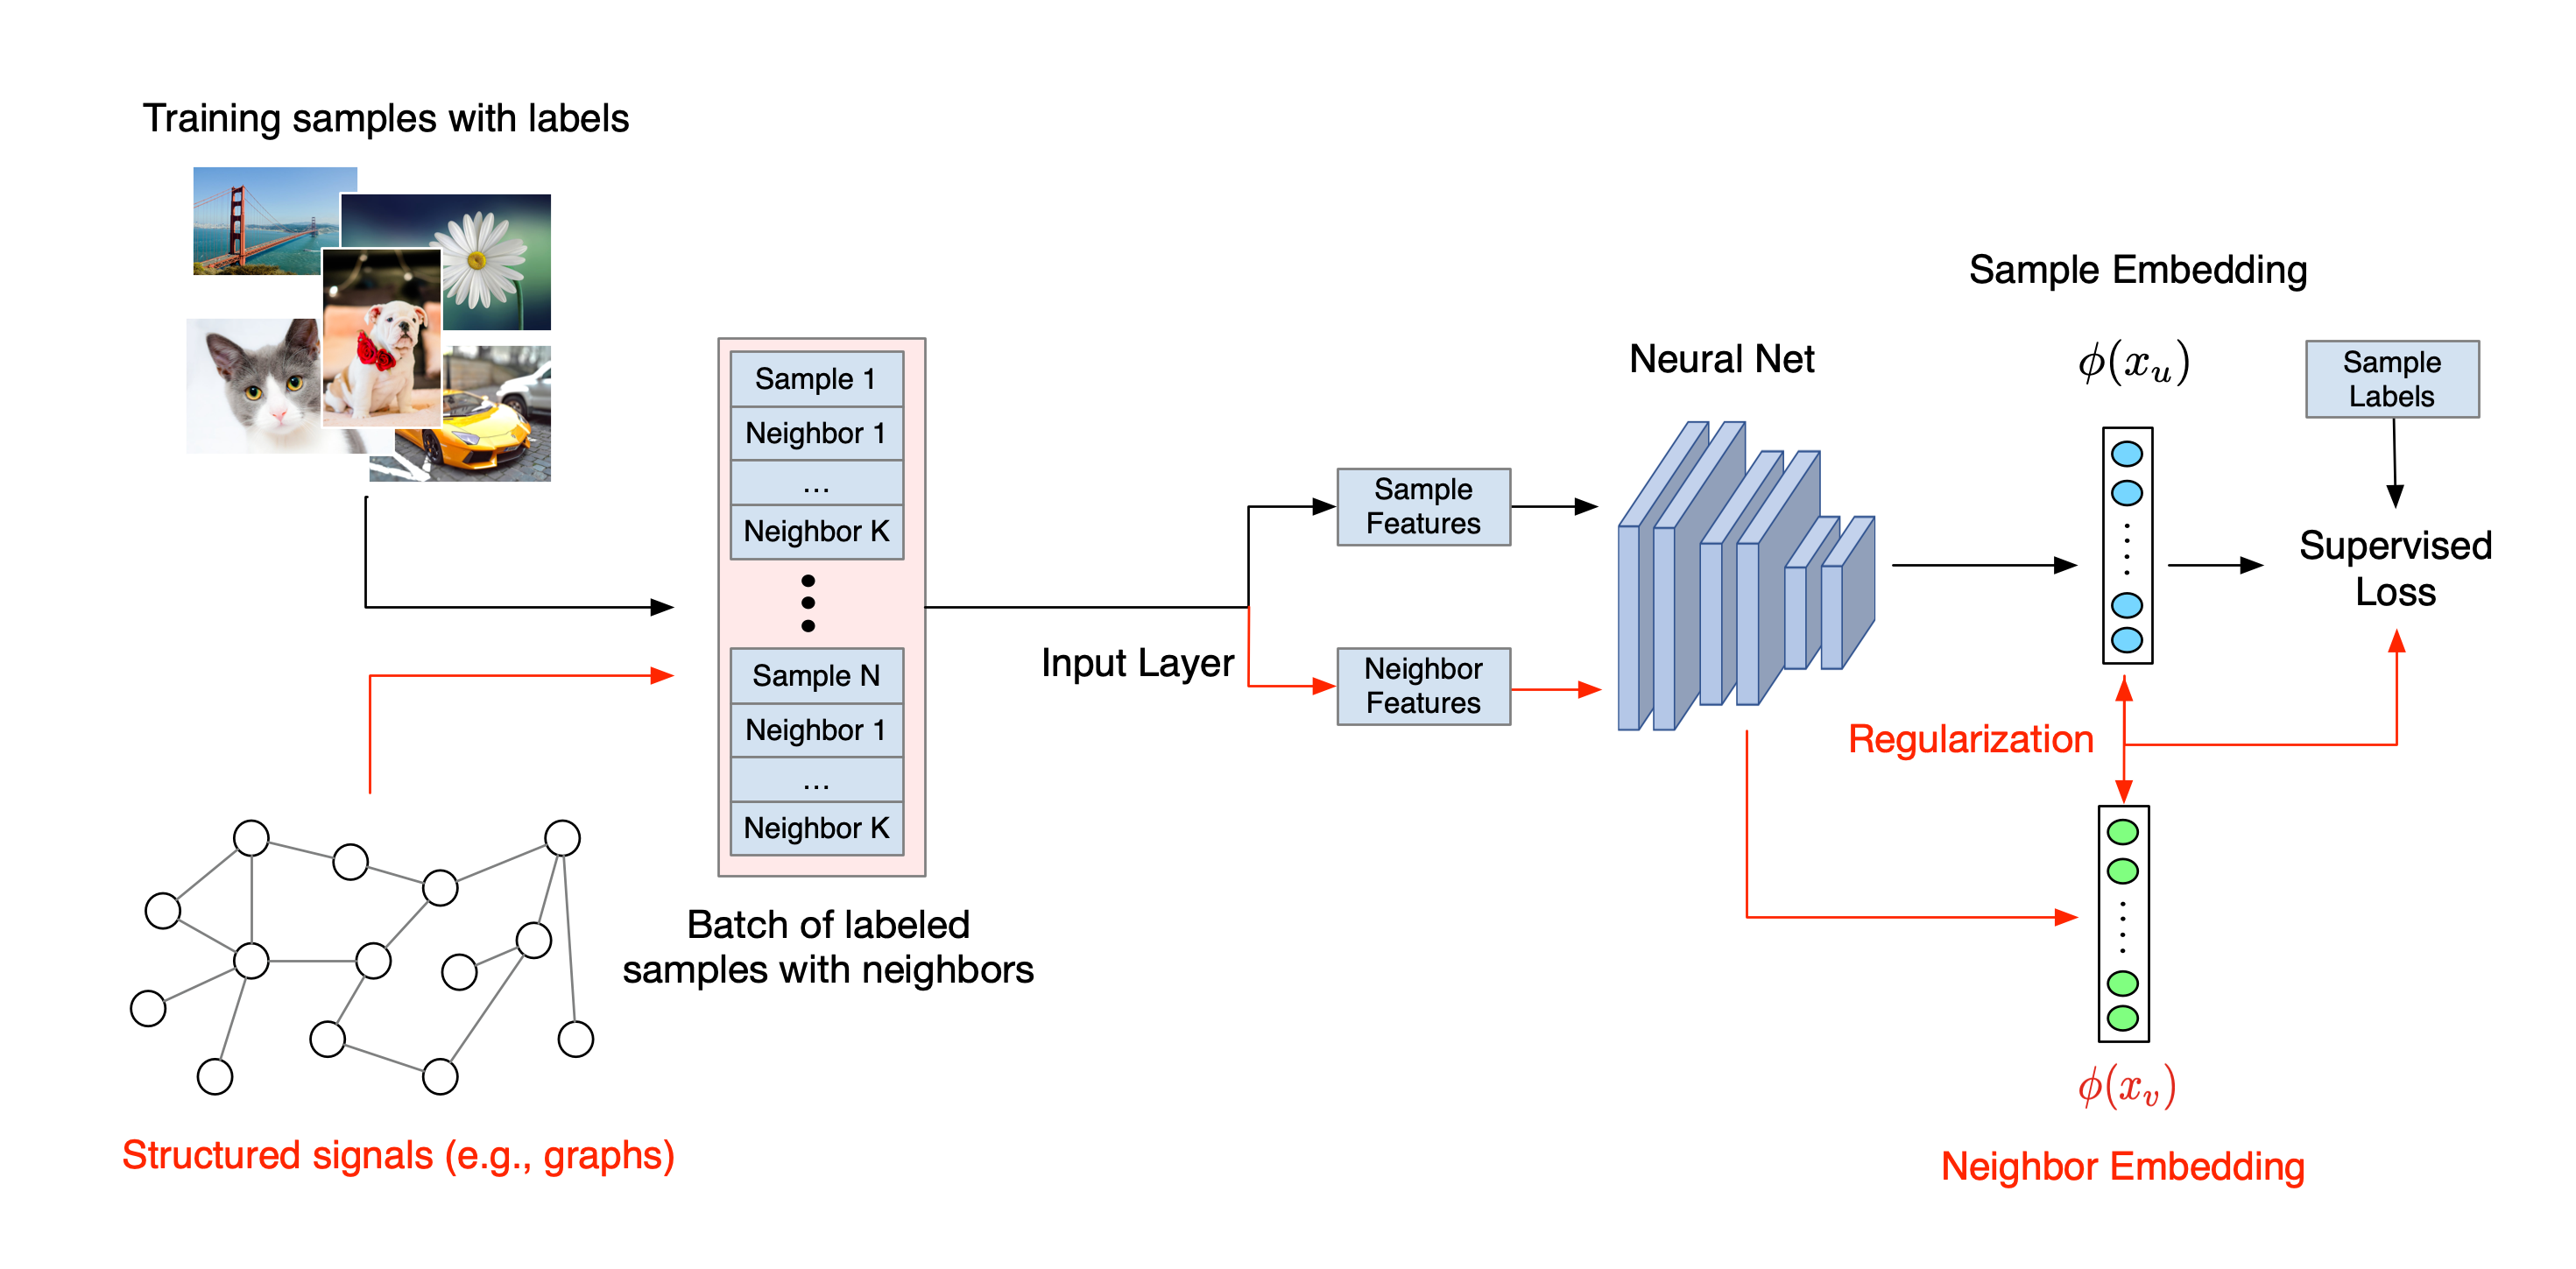
\includegraphics[width=0.8\linewidth]{Image/NSL.png}
    \caption {Neural Structured Learning}
    \label{Hình 1.2: Neural Structured Learning}
    \cite*{WEBSITE:4}
\end{figure}

Trong Neural Structured Learning (NSL), các tín hiệu có cấu trúc dù được xác định rõ ràng dưới dạng biểu đồ hay được học ngầm dưới dạng cách ví dụ đối nghịch được 
được sử dụng để thường xuyên đào tạo mạng neural, buộc mô hình phải học các dự đoán chính xác (bằng cách giảm thiểu mất mát có giám sát), đồng thời duy trì sự giống nhau giữa các đầu vào từ 
cùng một cấu trúc(bằng cách giảm thiểu tổn thất lân cận). Kỹ thuật này là chung và có thể được áp dụng trên các kiến trúc neural tùy ý, chẳng hạn như Feed-Forward NNs, CNNs, RNNs. 


\subsection{Neural Graph Learning}

\textbf{Training with natural graphs}

\begin{figure}[h!]
    \centering
    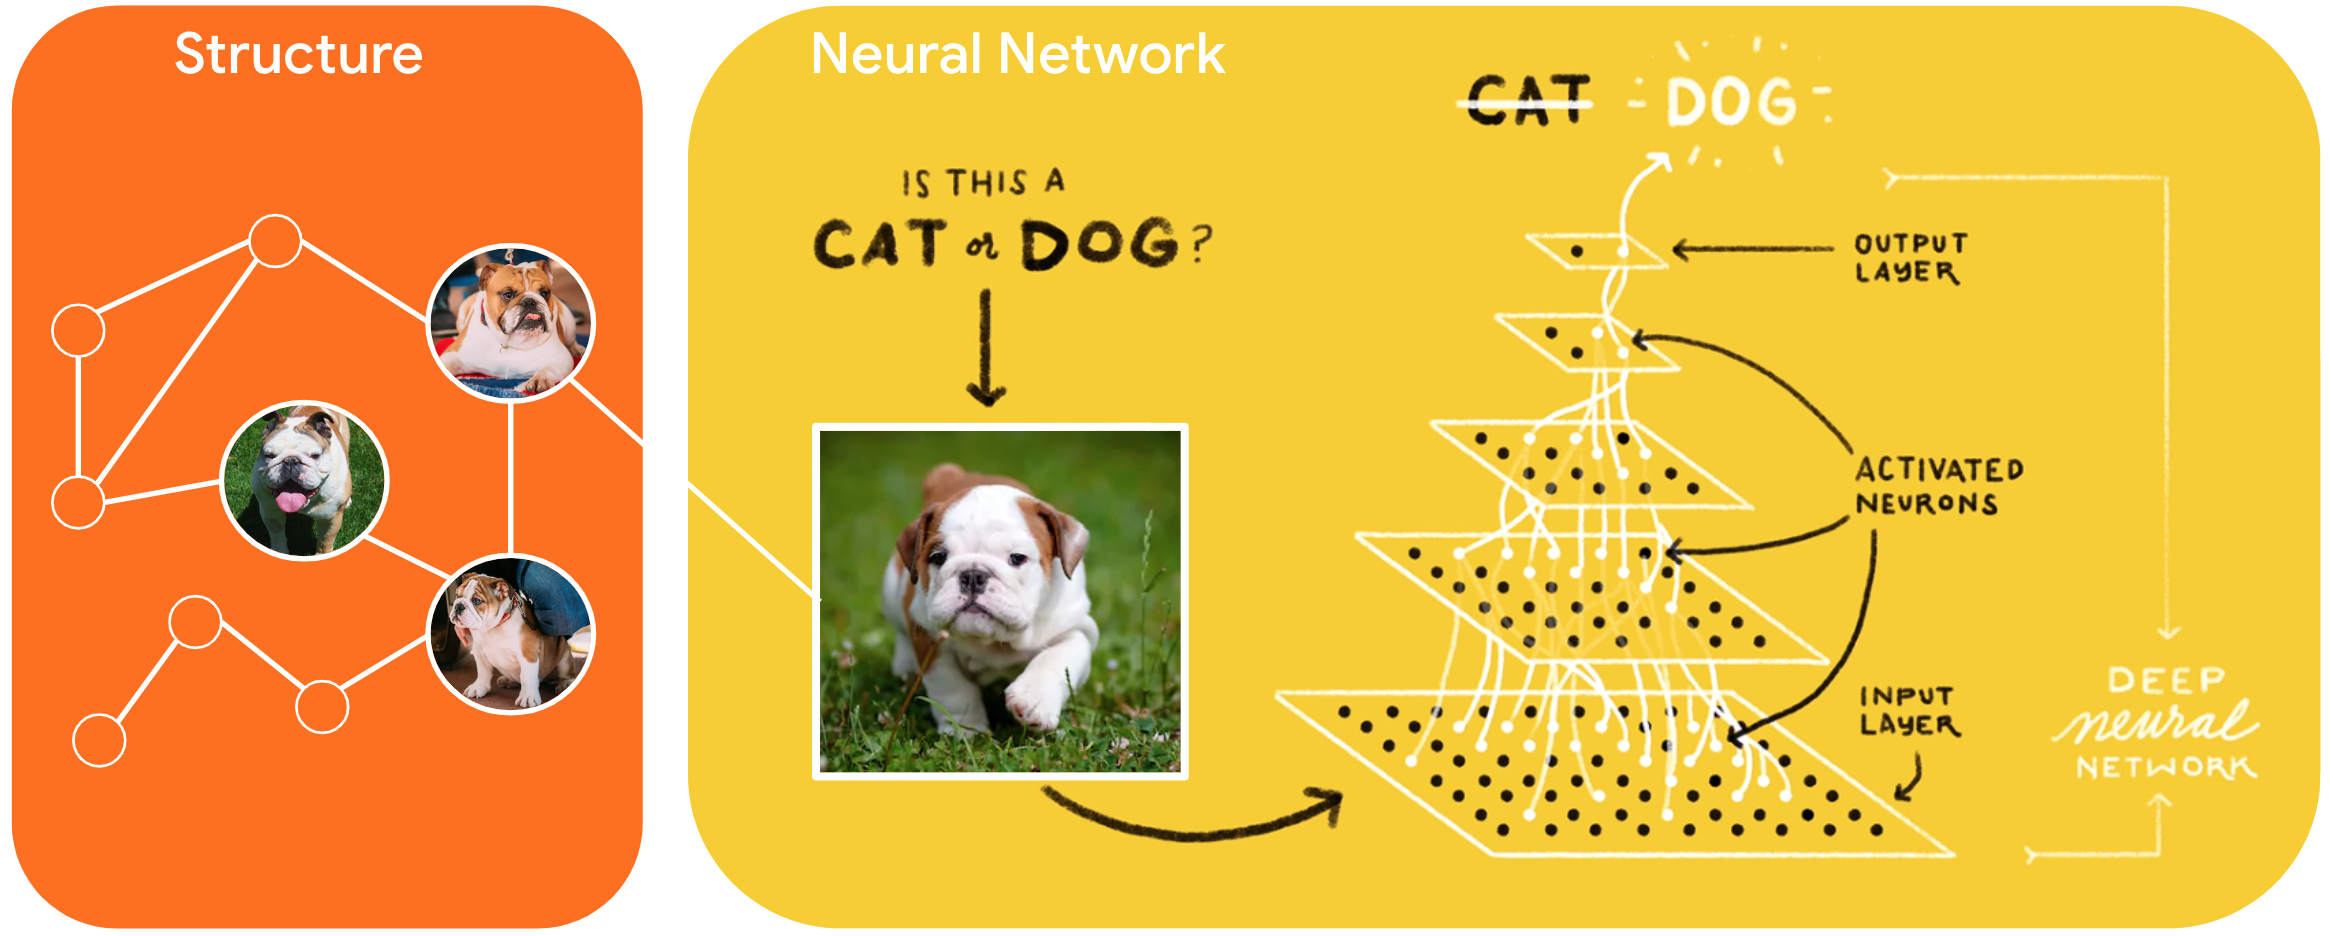
\includegraphics[width=0.8\linewidth]{Image/nsl_overview.png}
    \caption{Training with natural graphs}
    \label{Hình 1.3: Training with natural graphs}
    \cite*{WEBSITE:4}
\end{figure}

Về cơ bản, đồ thị tự nhiên là một tập hợp các điểm dữ liệu có mối quan hệ mật thiết với nhau, bản chất của mối quan hệ này có thể thay đổi dựa trên bối cảnh.
Mạng xã hội và Web là những ví dụ kinh điển mà chúng ta tương tác hàng ngày, ngoài những ví dụ này, chúng còn thường xuất hiện trong dữ liệu thường được sử dụng
cho nhiều nhiệm vụ học máy. Ví dụ khi ta cố gắng nắm bắt hành vi của người dùng dựa trên tương tác của họ với dữ liệu, thì việc lập mô hình dữ liệu dưới dạng biểu đồ 
có thể hợp lý. Đối với xử lý ngôn ngữ tự nhiên, chúng ta có thể định nghĩa một biểu đồ văn bản trong đó các nút biểu thị các thực thể và các cạnh biểu thị mối quan hệ 
giữa các cặp thực thể.

Xem xét bài toán phân loại tài liệu. Ví dụ như những kỹ sư AI thường chỉ quan tâm đến các bài viết về học máy trên một chủ đề cụ thể như thị giác máy tính hoặc xử lý ngôn ngữ
tự nhiên hoặc học tăng cường. Và thông thường, chúng ta có rất nhiều tài liệu hoặc giấy tờ như thế để phân loại, nhưng rất ít trong số chúng có nhãn. Vì vậy cần phải làm cho 
dữ liệu được thiết lập thành một biểu đồ tự nhiên, điều này nghĩa là nếu một bài báo hoặc tài liệu được trích dẫn từ bài báo hoặc tài liệu khác thì chúng có thể có cùng nhãn.
Việc sử dụng các thông tin quan hệ như vậy từ biểu đồ trích dẫn tận dụng được cả các mẫu được gắn nhãn cũng như không được gẵn nhãn. Điều này có thể bù đắp cho việc thiếu nhãn 
trong dữ liệu đào tạo. Vì vậy, việc xây dựng các đồ thị tự nhiên là rất cần thiết để giúp đào tạo các mô hình học máy một cách hiệu quả hơn.

\textbf{Traning with synthesized graphs}

\begin{figure}[h!]
    \centering
    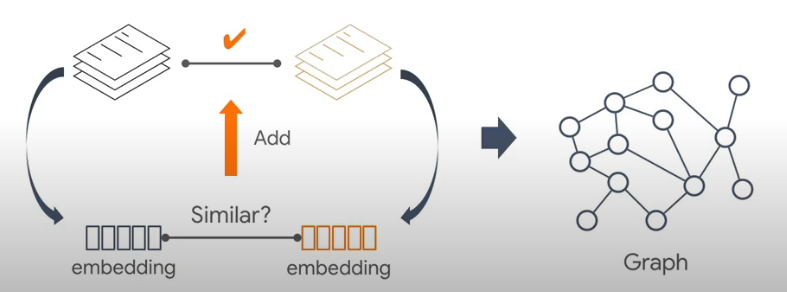
\includegraphics[width=0.8\linewidth]{Image/Graph2.png}
    \caption{Traning with synthesized graphs}
    \label{Hình 1.3: Traning with synthesized graphs}
    \cite*{WEBSITE:4}
\end{figure}

Mặc dù đồ thị tự nhiên là phổ biến, tuy nhiên có nhiều bài toán học máy với dữ liệu đầu vào không tạo thành đồ thị tự nhiên.
Ví dụ như phân loại văn bản đơn giản hoặc phân loại hình ảnh thì dữ liệu đầu vào chỉ chứa hình ảnh hoặc văn bản thô, do đó ta không thể 
tạo ra biểu đồ tự nhiên. Vì vậy Training with synthesized graphs được sử dụng để giải quyết vấn đề này. Với ý tưởng chính là xây dựng hoặc tổng hợp một biểu đồ từ dữ liệu đầu vào.
Trong Training with synthesized graphs chúng ta vẫn sự dụng sự giống nhau giữa các dữ liệu để xây dựng biểu đồ. Để xác định số liệu tương tự, thì cần phải chuyển đổi các văn bản thô hoặc
hình ảnh thành các thành phần nhúng tương ứng hoặc các biểu diễn dày đặc. Khi chuyển đổi dữ liệu thành các thành phần nhúng tương ứng, thì ta có thể sử dụng các mô hình đào tạo trước đó hoặc 
một số hàm chẳng hạn như cos để so sánh mức độ tương ứng giữa của các cặp phần nhúng. Nếu điểm tương đồng lớn hơn một ngưỡng nhất định thì ta sẽ thêm vào một cạnh tương ứng vào biểu đồ kết quả.
Việc lặp lại quy trình này sẽ bao phủ toàn bộ tập dữ liệu và sẽ tạo ra một biểu đồ. Và khi ta có biểu đồ thì việc sử dụng phương pháp học có cấu trúc trung tính rất đơn giản.


\subsection{Adversarial Learning}

\subsubsection*{Adversarial examples}

Adversarial example là các mẫu được tạo ra với những thao tác tinh vi bằng cách thêm vào các nhiễu đối nghịch nhỏ mà mắt người không thể nào nhìn thấy được đã biến nó thành một hình ảnh hoàn toàn khác dưới con mắt kỹ thuật số của thuật 
toán machine learning.

Một số mô hình học máy bao gồm các mạng lưới thần kinh hiện đại nhất, dễ bị sai lệch trước những Adversarial examples. Những mô hình này cho ra kết quả sai các ví dụ chỉ khác một chút so với các ví dụ được phân loại chính xác từ trong tập 
dữ liệu. Ví dụ như khi chúng ta đưa ra đặc điểm của một con gấu trúc thì chúng ta sẽ tìm những đặc trưng của nó như mắt đen, đầu tròn, thân trắng... Nhưng đối với một mạng neural nhân tạo, miễn là khi dữ liệu được đưa vào chạy qua các layer 
đưa ra kết quả trả lời đúng thì nó sẽ tin hình ảnh của dữ liệu đó là con gấu trúc.

\begin{figure}[h!]
    \centering
    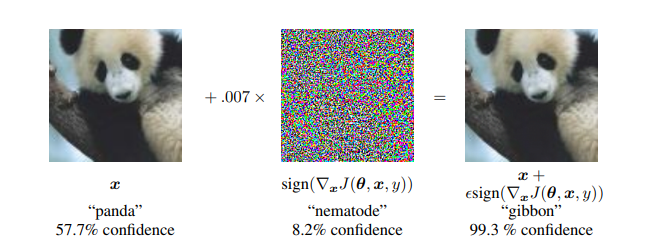
\includegraphics[width=0.8\linewidth]{Image/ADV.png}
    \caption{Adversarial examples}
    \label{Hình 1.4: Adversarial examples}
    \cite*{Reference7}
\end{figure}

Từ hình 2.4 ta thấy, khi thêm vào 1 vector tín hiệu nhiễu rất rất bé mà mắt người không thể phân biệt được sự khác nhau giữa hai hình ảnh của con gấu trúc thì nó đã đánh lừa được mạng neural và khiến nó phán đoán sai và nó tin chắc rằng
thứ mà nó đang nhìn thấy là con vượn (99.3\%). Điều này cho thấy khi các tập dữ liệu không tốt(có nhiễu) thì có thể khiến mạng neural đưa ra phán đoán sai.
 Để giải quyết vấn đề này, Adversarial training được đề xuất để dạy các mạng neural không bị đánh lừa và phân loại sai. 

\cite*{Reference6}
\textbf{Adversarial training}

Khái niệm về Adversarial training liên quan đến việc đào tạo bộ phân loại để khái quát hóa
Adversarial examples cũng như mẫu sạch. Trong lược đồ đào tạo thông thường, được hiển thị trong Hình 2.5, dữ liệu đào tạo chuyển tiếp
thông qua mô hình và tổn thất dự đoán được lan truyền ngược để cải thiện phân loại
kết quả. Kết quả là, mô hình sẽ khái quát hóa việc phân phối dữ liệu huấn luyện để
đưa ra một dự đoán chính xác về nhãn. 

Để đào tạo mô hình tránh bị nhầm lẫn khi tập dữ liệu có nhiễu thì ta sẽ tạo ra các dữ liệu có nhiễu nhỏ từ tập dữ liệu đào tạo
sau đó thêm các cạnh để kết nối dữ liệu vừa tạo ra với các mẫu của nó để xây dựng một cấu trúc linh hoạt sau đó, cấu trúc này có thể được sử dụng trong khung học tập
của cấu trúc thần kinh. Trong khung học cấu trúc thần kinh, mạng thần kinh cố gắng học cách duy trì cấu trúc bằng cách giữ sự giống nhau giữa một mẫu và hàng xóm của nó.
 Vì vậy về cơ bản việc sử dụng tập dữ liệu sạch và dữ liệu đối nghịch của nó sẽ nói với mạng thần kinh rằng mẫu và mẫu đối nghịch của nó thực sự giống nhau. Vì vậy, hãy giữ sự 
 giống nhau giữa chúng và đừng bị nhầm lẫn bởi các nhiễu.

\begin{figure}[h!]
    \centering
    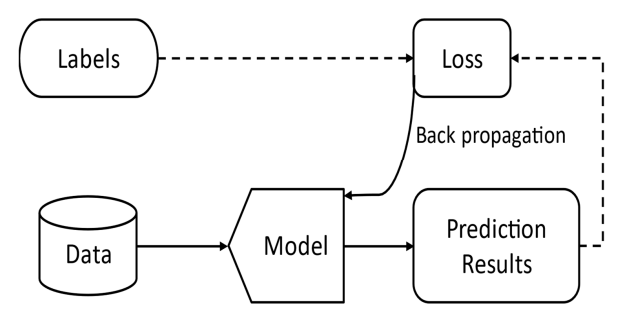
\includegraphics[width=0.72\linewidth]{Image/ADVT1.png}
    \caption{Basic training}
    \label{Hình 2.5: Adversarial training}
    \cite*{Reference8}
\end{figure}

Adversarial training mở rộng các phương pháp đào tạo thông thường bằng cách bổ sung thêm
bước vào quy trình đào tạo, như được minh họa trong Hình 2.6. Bằng cách này, mô hình có thể
khái quát hóa cả dữ liệu sạch và dữ liệu đối nghịch được tạo ra bởi các phương thức
được sử dụng trong Adversarial training để chống lại sự đánh lừa của mẫu đối nghịch.

\begin{figure}[h!]
    \centering
    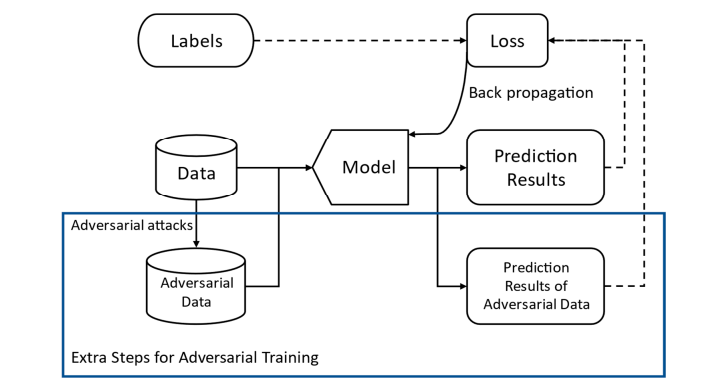
\includegraphics[width=0.72\linewidth]{Image/ADVT2.png}
    \caption{Adversarial training}
    \label{Hình 2.6: Adversarial training}
    \cite*{Reference8}
\end{figure}

Trong thư viện TensorFlow có sẵn các hàm chức năng để tạo ra các mẫu đối ngịch. 
Tương tự thì Keras API cũng có thể sử dụng để cho phép đào tạo từ đầu đến cuối
một cách dễ dàng với Adversarial training như: AdversarialRegularization, AdvNeighborConfig, AdvRegConfig...

\section{Adversarial Regularization for Image Classification}
\subsection{Chuẩn bị dữ liệu}

Ở phần trước chúng ta đã đi qua tổng quan về TensorFLow và Neural Structured Learning. Tuy nhiên để làm rõ hơn về hiệu quả của Neural
Structured Learning, chúng ta cần thực nghiệm trên một bài toán thực tế. Vì vậy ta sẽ ứng dụng Neural Structured Learning và chính xác hơn là Adversarial 
Regularization for Image Classification.
\begin{figure}[h!]
    \centering
    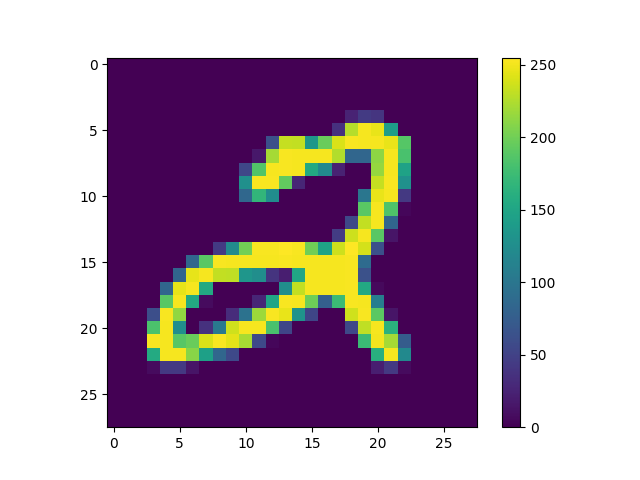
\includegraphics[width=0.6\linewidth]{Image/data.png}
    \caption{Ảnh chữ số viết tay được lấy từ tập dữ liệu MNIST}
    \label{Hình 2.7: GẢnh chữ số viết tay được lấy từ tập dữ liệu MNIST}
\end{figure}


Dựa trên tập dữ liệu có sẵn của thư viện TensorFlow MNIST, chúng ta sẽ thực hiện một bài toán phân loại ảnh chữ số viết tay. Tập dữ liệu bao gồm 70.000 ảnh
chữ số viết tay được chia thành 60.000 ảnh để huấn luyện và 10.000 ảnh để kiểm tra. Mỗi ảnh có kích thước 28x28 pixel và được biểu diễn dưới dạng một mảng
2 chiều 28x28. Mỗi phần tử trong mảng này là một giá trị từ 0 đến 255 biểu diễn độ sáng của một pixel. Để thuận tiện cho việc huấn luyện, chúng ta sẽ chuyển đổi
mỗi ảnh thành một mảng 1 chiều 784 phần tử. Để đơn giản hơn, chúng ta sẽ chia tập dữ liệu thành 2 tập huấn luyện và kiểm tra. Tập huấn luyện sẽ bao gồm 60.000 ảnh 
và tập kiểm tra sẽ bao gồm 10.000 ảnh. Mỗi ảnh sẽ được gán nhãn là một số từ 0 đến 9 tương ứng với chữ số viết tay. 

\subsection{Mô hình}
Chúng ta có thể sử dụng các mạng neural thông thường để xây dựng mô hình phán đoán chữ số. Ý tưởng là sử dụng một vài mạng neural để tính toán các trọng số
của mô hình. 
\begin{equation}
    \begin{aligned}  
      w_1X_1 + w_2X_2 + ... + w_nX_n = y\\
    \end{aligned}
\end{equation}

trong đó:
\begin{itemize}
    \item $w_1, w_2, ..., w_n$ là các trọng số của mô hình.
    \item $X_1, X_2, ..., X_n$ là giá trị của các pixel.
    \item $y$ là giá trị dự đoán của mô hình.
\end{itemize}


Mô hình sẽ tìm kiếm các trọng số phù hợp để đưa ra được đầu ra y chính xác đối với các hình ảnh đầu vào.
Tuy nhiên nếu thưc hiện như vậy, chúng ta sẽ không thể đạt được kết quả tốt. Vì vậy chúng ta cần phải sử dụng một số kỹ thuật để cải thiện độ chính xác của mô hình.
Bằng cách thêm các convolutional layer và pooling layer vào mô hình, chúng ta sẽ có thể giảm số lượng tham số của mô hình và cải thiện độ chính xác của mô hình.



Chúng ta sẽ thực hiện xây dựng và đào tạo một mạng neural đơn giản và một mạng neural sử dụng Adversarial Regularization. Sau đó chúng ta sẽ so sánh kết quả 
dự đoán của 2 mạng neural này để thấy được hiệu quả của Neural Structured Learning. Sau khi đào tạo và dự đoán thử trên tập dữ liệu có sẵn của TensorFlow, thì
ta sẽ thử viết tay một vài chữ số và để cho mạng neural dự đoán xem nó có thể dự đoán chính xác không.

Với những thư viện đồ sộ và khả năng làm việc với các ma trận tốt, Python là ngôn ngữ được lựa chọn để thực hiện ý tưởng trên. Cùng với đó là các thư viện như numpy, matplotlib và
đặc biệt là TensorFlow với API keras và Neural structed learning.



